\chapter{Introdução}

Cada vez mais a robótica tem feito parte da sociedade atual. Um dos problemas
atuas da robótica é o planejamento em ambientes multiagentes dinâmicos, em que
ao menos um agente não é controlado. Um bom exemplo de um desses ambientes
dinâmicos é um jogo de futebol de robôs, onde um grupo de robôs é controlado por
uma IA e o outro grupo por outra IA independente.

Devido a alta complexidade desses ambientes, não é viável o planejamento
considerando diretamente as leis físicas. Como consequência, limita-se as ações
possíveis do robô no modelo utilizado no planejamento para que se possa simular
mais situações em tempo hábil, uma vez que o ambiente esta continuamente sujeito
a modificações. Entretanto, para que as simulações sejam válidas, o robô real
deve estar em sintonia com seu modelo. Com efeito, o robô real deve executar os
comandos conforme o robô simulado, caso o mesmo ambiente simulado seja
encontrado na prática.

\begin{figure}
  \centering
  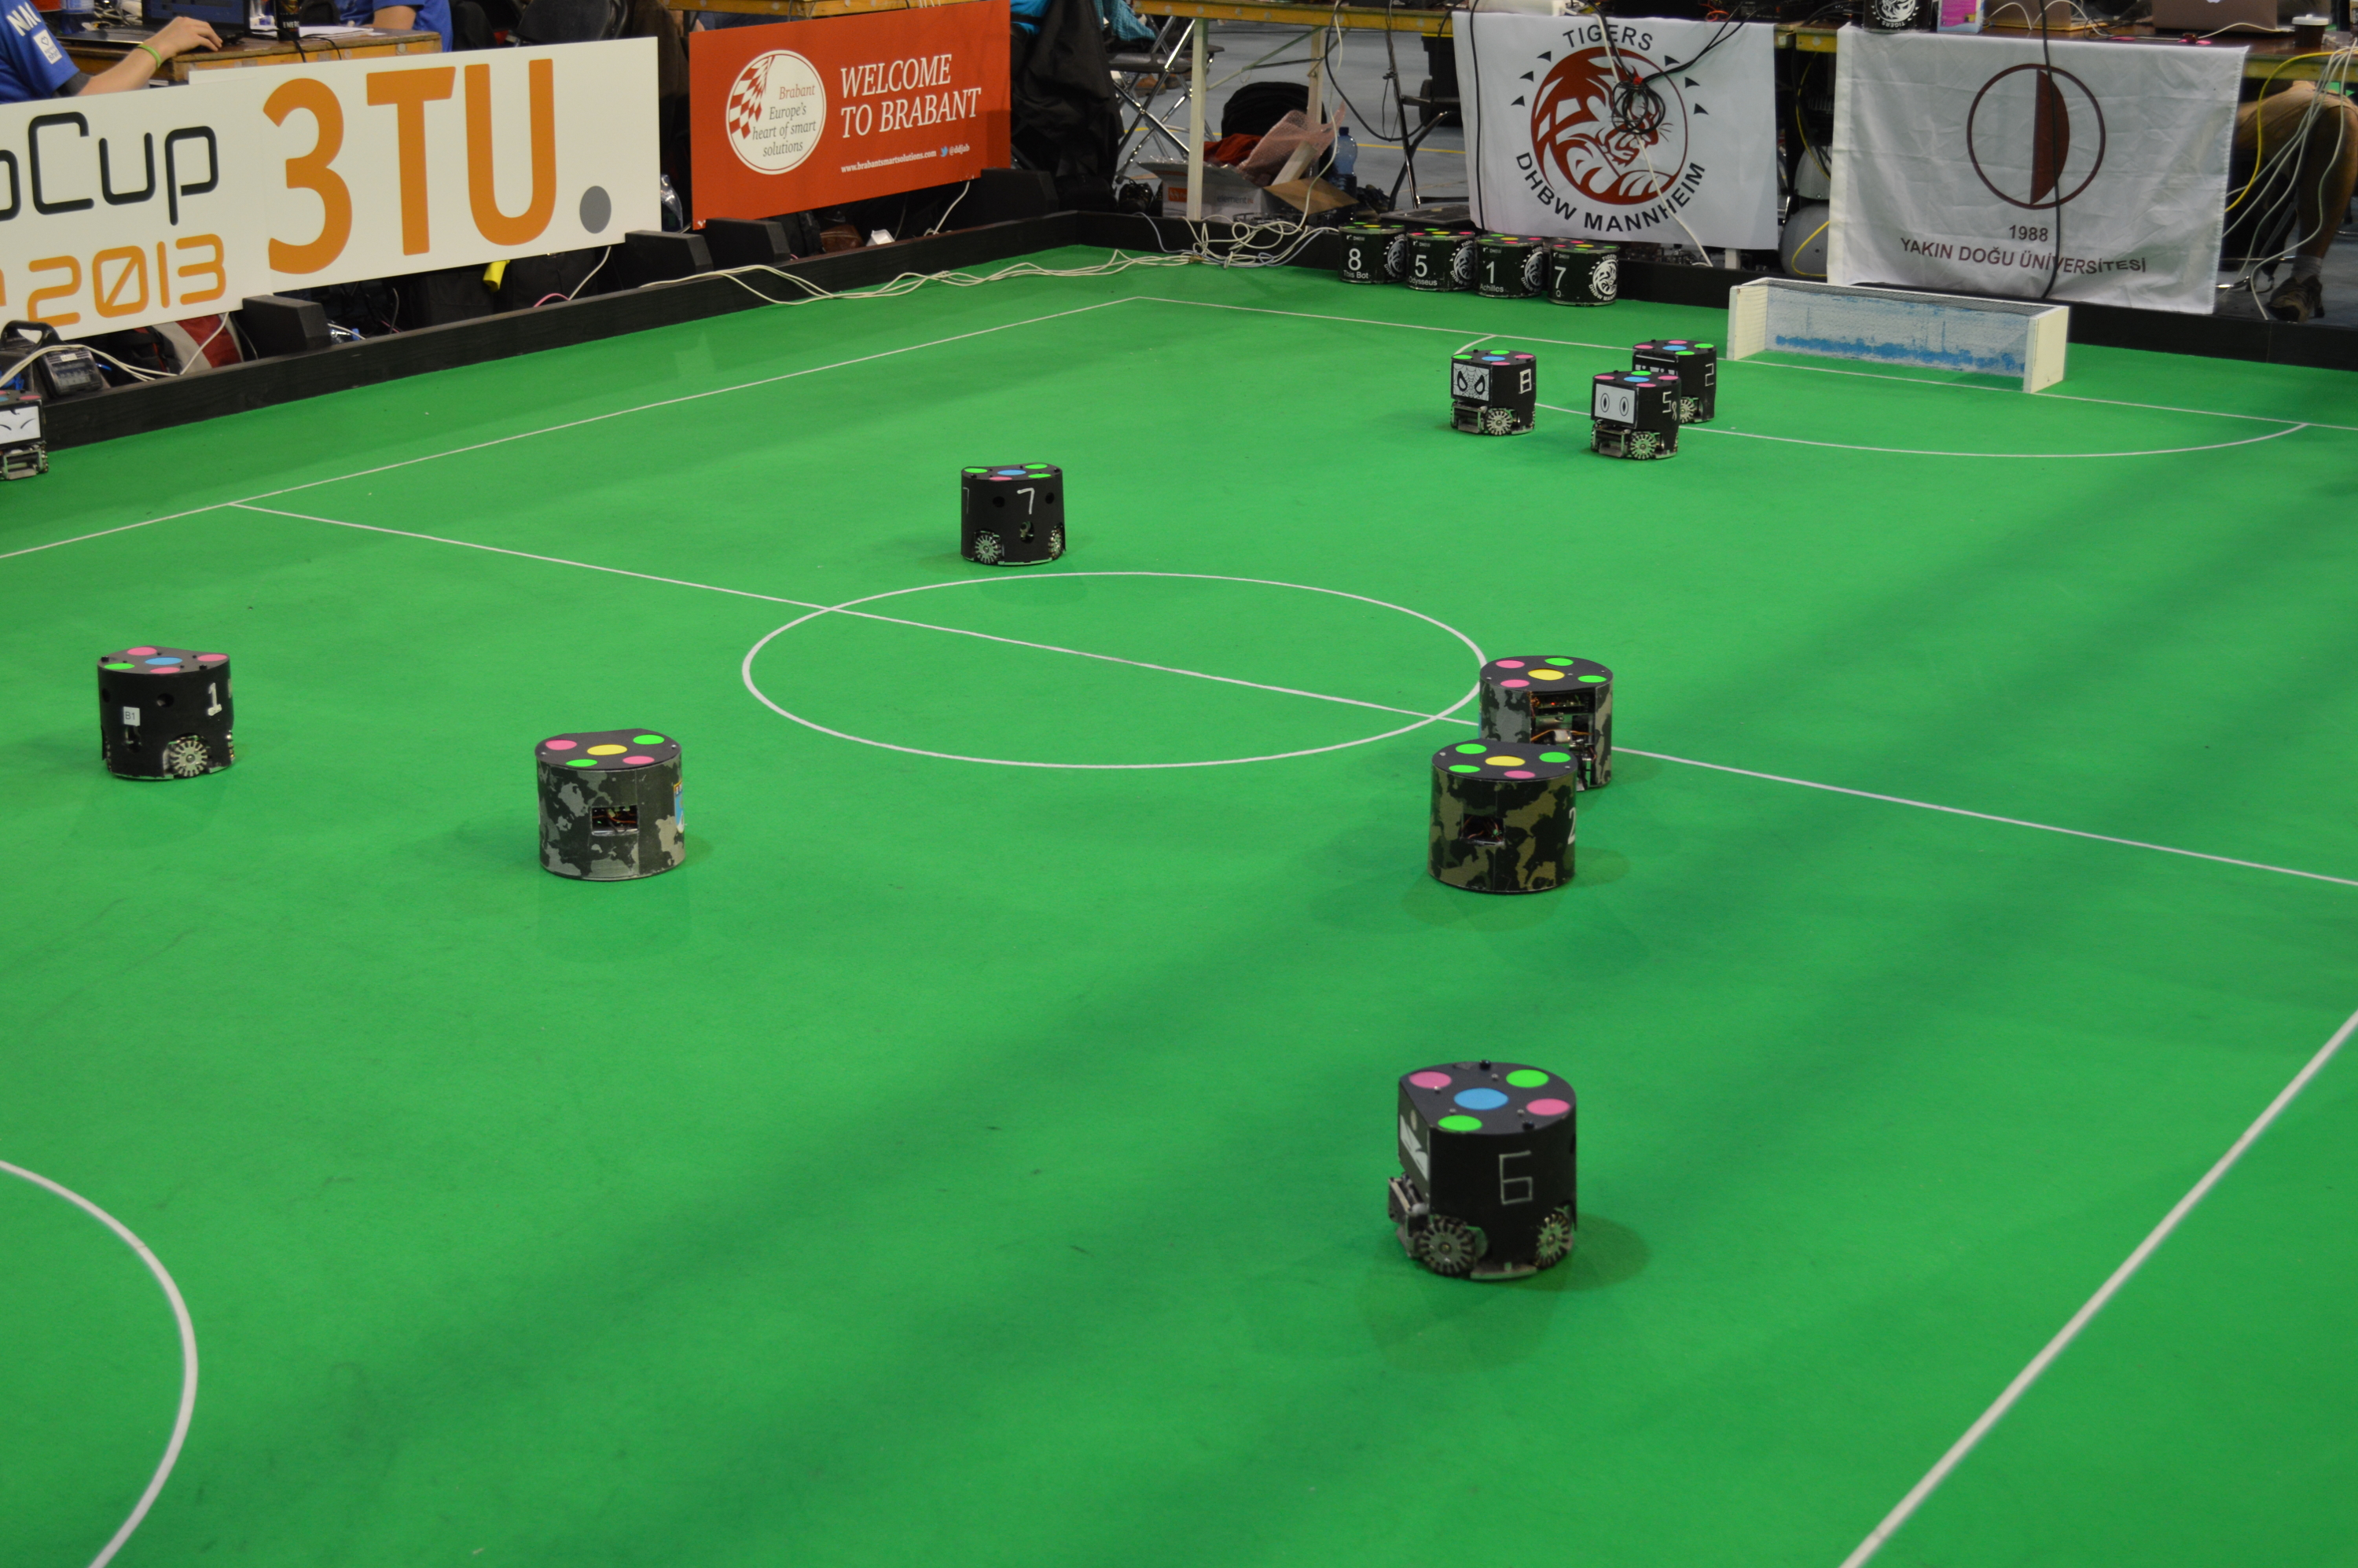
\includegraphics[width=0.8\linewidth]{robocup2013}
  \caption{Imagem da SSL \textit{RoboCup} 2013 em Eindhoven, na Holanda}\label{fig:robocup2013}
\end{figure}

A ideia de robôs jogando futebol foi mencionada pela primeira vez pelo professor
Alan Mackworth (University of British Columbia, Canadá) em um artigo intitulado
"On Seeing Robots", apresentado no Vision Interface 92 e posteriormente
publicado em um livro chamado Computer Vision: System, Theory and Applications.
Independentemente, um grupo de pesquisadores japoneses organizou um Workshop no
Ground Challenge in Artificial Intelligence, em Outubro de 1992, Tóquio,
discutindo e propondo problemas que representavam grandes desafios. Esse
Workshop os levou a sérias discussões sobre usar um jogo de futebol para
promover ciência e tecnologia. Estudos foram feitos para analisar a viabilidade
dessa ideia. Os resultados desses estudos mostram que a ideia era viável,
desejável e englobava diversas aplicações práticas. Em 1993, um grupo de
pesquisadores, incluindo Minoru Asada, Yasuo Kuniyoshi e Hiroaki Kitano,
lançaram uma competição de robótica chamada de Robot J-League (fazendo uma
analogia à J-League, nome da Liga Japonesa de Futebol Profissional). Em um mês,
vários pesquisadores já se pronunciavam dizendo que a iniciativa deveria ser
estendida ao âmbito internacional. Surgia então, a Robot World Cup Initiative
(RoboCup).

RoboCup é uma competição destinada a desenvolver os estudos na área de robótica
e Inteligência Artificial (IA) por meio de uma competição amigável. Além disso,
ela tem como objetivo, até 2050, desenvolver uma equipe de robôs humanoides
totalmente autônomos capazes de derrotar a equipe campeã mundial de futebol
humano. A competição possui várias modalidades. Neste trabalho, será analisada a
Small Size Robot League (SSL), também conhecida como F180. De acordo com as
regras da SSL de 2013, as equipes devem ser compostas por 6 robôs, sendo um deles o
goleiro, que deve ser designado antes do início do jogo. Durante o jogo, nenhuma
interferência humana é permitida com o sistema de controle dos robôs. É
fornecido aos times um sistema de visão global e esses controlam seus robôs com
máquinas próprias. O sistema de controle dos robôs geralmente é externo e recebe
os dados de um conjunto de duas câmeras localizadas acima do campo. Esse sis-
tema de controle processa os dados, determina qual comando deve ser executado
por cada robô e envia este comando através de ondas de rádio aos robôs. Embora
seja permitido que as equipes utilizem sistemas próprios de visão, a maioria das
equipes utiliza a visão centralizada. Uma arquitetura típica utilizada pelas
equipes da SSL é apresentada na figura~\ref{fig:arq_ssl}. A
figura~\ref{fig:robocup2013} mostra uma imagem da SSL Robocup 2013, da qual a
RoboIME (Equipe de Futebol de Robôs do Laboratório de Robótica do IME)
participou.

\begin{figure}
  \centering
  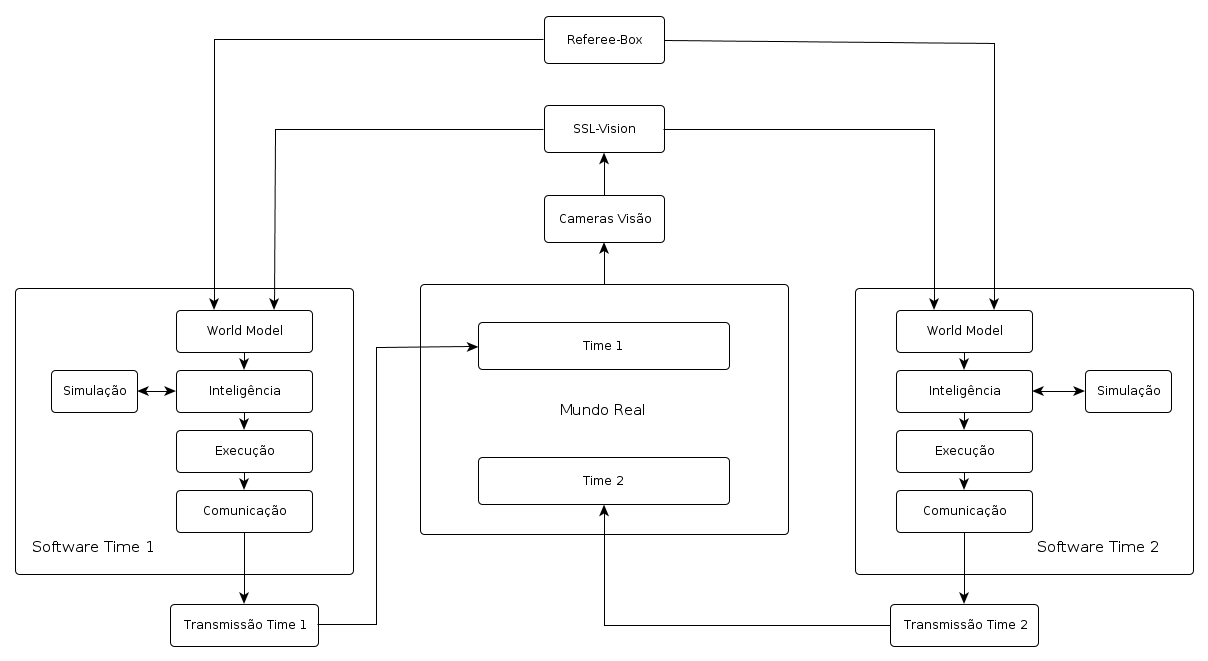
\includegraphics[width=0.8\linewidth]{arquitetura_ssl}
  \caption{Arquitetura típica da SSL}\label{fig:arq_ssl}
\end{figure}

\section{Motivação}

O futebol de robôs, problema padrão de investigação internacional, reúne grande
parte dos desafios presentes em problemas do mundo real a serem resolvidos em
tempo real. As soluções encontradas para o futebol de robôs podem ser
estendidas, possibilitando o uso da robótica em locais de difícil acesso para
humanos, ambientes insalubres e situações de risco de vida iminente.  Há
diversas novas áreas de aplicação da robótica, tais como exploração espacial e
submarina, navegação em ambientes inóspitos e perigosos, serviço de assistência
médica e cirúrgica, além do setor de entretenimento. Essas áreas podem ser
beneficiadas com o desenvolvimento de sistemas multi robôs. Nestes domínios de
aplicação, sistemas de multi robôs deparam-se sempre com tarefas muito difíceis
de serem efetuadas por um único robô.  Um time de robôs pode prover redundância
e contribuir cooperativamente para resolver o problema em questão. Com efeito,
eles podem resolver o problema de maneira mais confiável, mais rápida e mais
econômica, quando comparado com o desempenho de um único robô.

Devido a alta complexidade de sistemas multiagentes dinâmicos, torna-se
necessário um modelo simplificado para que sejam executadas o maior número de
simulações possível.  Caso seja possível uma discretização, ter-se-á um número
finito de casos para serem avaliados. Com isso, pode-se aplicar algoritmos como
o minimax (aplicados a jogos de competitivos de soma zero) para encontrar
soluções ao problema.

Isso é muito mais desejável que um modelo heurístico de IA, onde as soluções são
criadas com base nos ambientes identificados pelos modeladores. Isso, pois a
modelagem puramente heurística limita o número de jogadas que se pode executar e
limita a capacidade que o computador tem de testar um grande número de possibilidades.

\section{Objetivo}

O objetivo deste trabalho é desenvolver um algoritmo de controle para o futebol
de robôs que obtenha um desempenho melhor que o utilizado atualmente, de acordo
com um critério que será definido posteriormente.
Como objetivos secundários, este trabalho objetiva criar um modelo discreto para
o problema do futebol de robôs, que é um jogo contínuo de soma zero.
A partir desta discretização, pretende-se desenvolver uma arquitetura de
controle com base no algoritmo minimax para se planejar jogadas.

\section{Justificativa}
% TODO: incluir referências

Uma arquitetura de controle que simule os diversos ambientes dinamicamente de
maneira sequencial de um ambiente multiagente permite que várias jogadas sejam
criadas dinamicamente, diferentemente de uma arquitetura estática baseada em uma
heurística. Essa abordagem heurística é legada da maneira como estratégias são
planejadas nos times de futebol humano.

Com tal mecanismo é possível melhorar a IA em uso pela RoboIME
para tomar decisões que levem a resultados melhores e, como consequência, ganhar
mais partidas. Nenhuma equipe atualmente esta seguindo esta abordagem, mas os
autores acreditam que essa é uma linha de pesquisa promissora.

\section{Metodologia}

Para atingir os objetivos propostos será seguida a seguinte metodologia.
Inicialmente a teoria sobre jogos será revisada. São apresentados também
alguns dados empíricos observados com testes informais realizados anteriormente.

Em sequência, um modelo abstrato do futebol de robôs é proposto para que seja
aplicado o algoritmo minimax. A partir deste modelo uma arquitetura de controle
é desenvolvida.

Em seguida são definidas métricas para comparar a arquitetura anteriormente
utilizada com a arquitetura atual.

Finalmente são apresentadas as conclusões parciais do projeto.

\section{Estrutura}

No capítulo~\ref{cap:minimax}, a teoria dos jogos é revisada e são apresentados
alguns dados empíricos observados com testes observados anteriormente.
No capítulo~\ref{cap:mapeamento}, um modelo abstrato do futebol de robôs é
proposto.
No capítulo~\ref{cap:programa}, uma arquitetura de controle é desenvolvida com
base no modelo proposto anteriormente. Também são criadas métricas para
comparar os resultados obtidos com a nova arquitetura.
No capítulo~\ref{cap:cronograma}, o planejamento das próximas atividades é
apresentado.
No capítulo~\ref{cap:conclusao}, são apresentadas as principais conclusões
atingidas neste trabalho.
% vim: tw=80 et ts=2 sw=2 sts=2
